\documentclass[]{article}
\usepackage{graphicx}	
\usepackage{amssymb}
\usepackage{amsmath}
\usepackage{subfiles}
\usepackage{geometry}
\usepackage{braket}
\usepackage[table,xcdraw]{xcolor}
\usepackage{float}
\usepackage{hyperref}
\hypersetup{
    colorlinks=true,
    linkcolor=black,
    filecolor=cyan,      
    urlcolor=cyan,
    pdftitle={Phi Design},
}

\usepackage{listings}

\usepackage{amsthm}

\theoremstyle{definition}
\newtheorem{definition}{Definition}[section]
\usepackage{xcolor}

% \usepackage{arev}

% \usepackage{fontspec}
%     \setmainfont{SF Pro Text Regular}
%     \setmonofont{Fira Code Retina}

\usepackage{titlesec}
\titleformat{\chapter}[display]
  {\normalfont\huge}
  {\bfseries\chaptertitlename\ \thechapter}{20pt}{\Huge}

\titleformat{\section}
    {\normalfont\Large}
    {\thesection}{1em}{}

\titleformat{\subsection}
    {\normalfont\itshape\large}
    {\thesubsection}{1em}{}

\definecolor{codegreen}{rgb}{0.3,0.3,0.3}
\definecolor{codegray}{rgb}{0.5,0.5,0.5}
\definecolor{codepurple}{rgb}{0.69,0.69,0.69}
 
\lstdefinestyle{mystyle}{ 
    commentstyle=\color{codegreen},
    keywordstyle=\color{codegreen}\normalfont,
    numberstyle=\tiny\color{codegray},
    stringstyle=\color{codepurple},
    basicstyle=\ttfamily\footnotesize,
    breakatwhitespace=false,         
    breaklines=true,                 
    captionpos=b,                    
    keepspaces=true,                 
    numbers=left,                    
    numbersep=5pt,   
	tabsize=2,
    basicstyle=\ttfamily
}
 
\lstset{style=mystyle}


\usepackage{titling}
\renewcommand\maketitlehooka{\null\mbox{}\vfill}
\renewcommand\maketitlehookd{\vfill\null}

\title{\Huge The effects of weight distribution on flight time of rotocopters}
\author{\LARGE Rishi Kothari}
\date{Dichyant Thapa, Keesha Batra, Jessica Mathon \\ 23/02/2020 \\ SNC-1D8 \\ Mrs. Shabana Schwertner}

\geometry{margin=0.5in}

\begin{document}
\pagenumbering{gobble}
\maketitle

\newpage

\tableofcontents
\newpage

\pagenumbering{arabic}

\section{Definitions}
\begin{definition}{Wing Weight Ratio:}
    This is a ratio in the form $x:y$, where $x$ is the number of standard 0.03g staples stapled to the left wing of a rotocopter, and $y$ is the number of standard, 0.03g staples stapled to the right wing of that same rotocopter, satisfying $x + y = 8$. The phrase "decreased wing weight ratio" refers to the value of $\frac{x+1}{y-1}$, and the opposite is true for the phrase "increased wing weight ratio". For instance, the phrase "decreasing the wing weight ratio, starting at 4:4" talks about all of the wing weight ratios in decreasing order: (4:4, 3:5, 2:6, 1:7, 0:8). Note that the number of staples on each wing only changes by 1 each time.
\end{definition}

Please note that unless otherwise stated, all integer values in this paper denote the number of standard, 0.03g staples (i.e. "The wing weight ratio 3:4" can also be read as "The ratio of the additional weight added onto the left wing to the additional weight added onto the right wing of 3:4, in terms of 0.03g staples")

\section{Research Question}
How does altering the distribution of weight on a rotocopter's wings (between the left-to-right-wing-weight ratios ranging from $1$ to $>0.14$), measured in terms of grams, affect the total flight time of the rotocopter, measured in terms of seconds from the instant that the rotocopter is dropped from its initial height of 2.5m to the the time that the rotocopter touched the floor?

\section{Introduction}
One of the fundamental underpinnings of our world is the idea of flight; the world would not have become as accessible as it is today had there not been the breakthrough discoveries of thrust, lift, drag, and gravity. As our understanding of these factors changed, so too have our vehicles. Humans were able to engineer complex devices like the helicopter, airplane, and hybrids of these devices, and were able to change the ways that flight change. Focusing on the helicopter specifically, some of the properties that have been discovered to change the way that the object flies include the rounding of the wing, sharpness of a wing's rear edge, as well as wing tilt ("Factors affecting Lift"). Each of these properties link back to the 4 main points, as discussed before, and are simply physical features that affect these mathematical factors. However, the experimenters' interests were piqued when they looked at an image of a helicopter's rotor blades. The blades seemed to be drooping on one side, but remained upright on the other, showing a difference in weight for both of the rotor wings. This begged the question: why does this happen, and how does it affect the helicopter? This experiment is the result of that question, and will explore how the weight distribution of staples on a winged rotocopter will affects its flight.

\section{Purpose}
The purpose of this experiment to understand the effects of weight distribution on flight time within the context of rotocopters. Using a total of 8 staples for each measurement and shifting the ratio of staples per wing will give a greater understanding of how weight \textit{placement} affects flight, as opposed to merely the weight itself. In general, this experiment will also help develop a basic understanding of real-world flight factors, such as the mechanics behind airplane turning and helicopter lift.

\section{Hypothesis}
It is hypothesized that if the wing weight ratio of the rotocopter is decreased, then the time taken for the rotocopter to fly from its starting point 2.5m above the ground to the ground will decrease as well. 


\subsection{Justification}\label{Hypothesis Justification}
This experiment's testing procedure mimics the way that weight is distributed among the two wings of an aircraft.

The weight distribution across the wings of the rotocopter will be changed by taking a certain amount of weight from one wing and adding it to the other, which mimics the manner in which a winged aircraft normally turns.

Taking the example of a simple biplane, turning is not achieved by rotating about the 'z' axis, as a car would, but rather by turning about the 'x' axis, using a technique known as 'banking'.

In order to turn an airplane, flaps on the wings known as ailerons are rotated , which affects the airflow passing over the wing. This modified airflow creates a pressure differential above and below the wing in question, which can create or take away lift. This idea can be thought of as putting weight on a certain wing, allowing the airplane to turn, as can be seen in Figure \ref{Banked Turn}.

\begin{figure}[H]
    \centering
    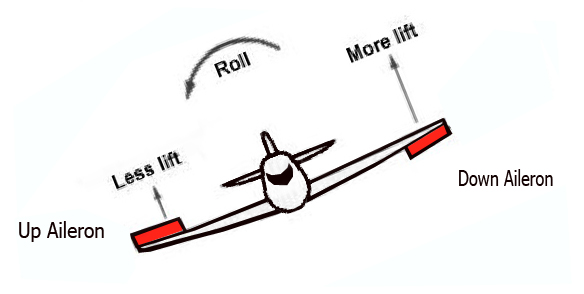
\includegraphics[scale=0.5]{graphics/aileron.jpg}
    \caption{A demonstration of how changing the angles of the ailerons affects the roll of an airplane, allowing it to turn}
    \label{Banked Turn}
\end{figure}

However, changing the angle of the flight is not the only effect banking has on an airplane's angle: it also decreases the \textit{total} amount of lift on the airplane.

See, as the airplane rolls to one direction, its lift vector moves with it(Cutler 2019), as can be seen in Figure \ref{Banking Lift}:

\begin{figure}[H]
    \centering
    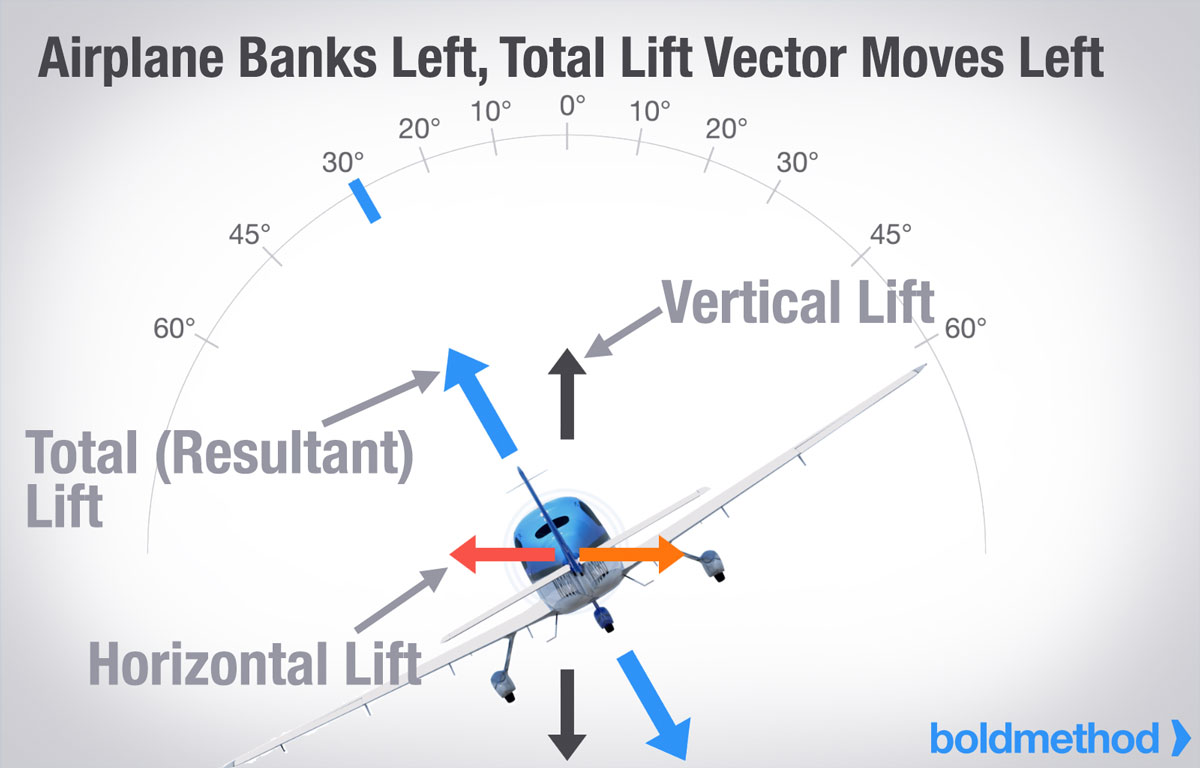
\includegraphics[scale=0.25]{graphics/bank-left.jpg}
    \caption{The effect that banking has on an aircraft's total lift}
    \label{Banking Lift}
\end{figure}

This means that as an airplane rolls, its altitude decreases correspondingly (Cutler 2019), as the total lift on the airplane is no longer facing upwards. In order for the airplane's altitude to stay constant, more speed must be applied to it, so that more airflow can be applied to the wings, and thus creating lift. In essence, as the bank of an aircraft changes, the speed increases(Cutler 2019). 

This same principle can be applied to this experiment, as in order to change the weight distribution of a rotocopter, weight must be taken from one wing and added to the other(Cutler 2019). This is much like the way that an airplane banks, but using physical weights as opposed to air. As a result, it can be assumed that the 'bank' angle of the rotocopter will change in correlation with a decrease in the ratio of the weights of the rotocopter's wings (i.e. a rotocopter with weight ratio 4:4 would be perfectly level, but a rotocopter with weight ratio 0:8 would heavily lean towards the side).

Just as the increase of a bank angle in an aircraft causes a corresponding change in the speed of that aircraft, it can also be assumed that this property follows through in rotocopters as well.

As stated previously, a rotocopter with weight ratio 4:4 would be level, but a rotocopter with weight ratio 0:8 would heavily lean towards the side, indicating a negative linear relationship\footnote{Note that it is assumed to be linear because all the possible shifts in the wing weight ratio (4:4, 3:5, 2:6, 1:7, etc.) all have equal increments, which follow a linear pattern} between the amount of time taken to fly from the starting point to the ground and the wing weight ratio; as the wing weight ratio decreases, the speed increases, which decreases the amount of time taken to cross a given distance.

\section{Variables}

\begin{table}[]
    \begin{tabular}{lll}
    Independent &
      Standardized &
      Dependent \\
    - Wing weight ratio of rotocopter &
      \begin{tabular}[c]{@{}l@{}}- Height of Rotocopter Starting point\\ - Material choice \& Dimensions of Rotocopter\\ - Prescence of Air Drafts\\ - Proximity of Rotocopter to Wall\end{tabular} &
      \begin{tabular}[c]{@{}l@{}}- The total amount of time the rotocopter\\ spent in the air, measured in seconds\\ from the moment that the rotocopter\\ was dropped from its starting point 2.5m\\ above ground, to the point in time at\\ which any part of the rotocopter was touching\\ the chosen ground.\end{tabular}
    \end{tabular}
    \caption{Summary of Variables}
    \label{variables}
    \end{table}

\label{independent}
\subsection{Independent}
The only part of the experiment that is being changed is the wing weight ratio of each rotocopter. This value represents the ratio of the amount of standard 0.03g staples on the left wing of the rotocopter to the amount of standard 0.03g staples on the right wing of the rotocopter.

In order to modulate this variable, for each trial, the number of staples on the left wing was decreased by one, and the number of staples on the right wing was increased by 1, starting with a control group of 4:4.

\subsection{Dependent}
The total amount of time the rotocopter spent in the air, measured in seconds from the moment that the rotocopter was dropped from its starting point $2.5 \pm 0.1$m above ground, to the point in time at which any part of the rotocopter was touching the chosen ground.

\subsection{Standardized}

\subsubsection{Height of Rotocopter starting point}
The measured flight time is the total amount of time that it takes for a given rotocopter to travel from its starting point at 2.5m in the air to the ground. If this variable is changed, then flight times will be changed for each trial, which skews the values.

\subsubsection{Material choice and dimensions of Rotocopter}
Every material has a certain density associated with it. This means that as the material is changed, the mass of the given rotocopter also changes. According to Newton's Second Law of Motion (recall $F=ma$), a greater mass will result in a \textbf{greater time to accelerate to the same speed}. By extension, this means that a rotocopter with a larger mass would have an ending speed lower than that of a regular mass, thus increasing the flight time for the larger one, and skewing the data in the process\footnote{The control group was designed with this fact in mind; the weight must be kept constant across all trials}. This necessitates the regulation of materials and dimensions.

\subsubsection{Prescence of air drafts}
The measured (dependent) variable of the experiment, in a general context, is the time taken for an object to fly from one point to another as a result of some change to the given object. Introducing a headwind or tailwind (two types of air drafts) would change the speed of the object unnaturally, which would lead to a lower or higher speed, respectively. This would cause the timing to be skewed, and requires the usage of a room that has little wind or contact with the outdoors.

\subsubsection{Proximity to wall}
In order to measure the time taken for any object to fall, the object must be able to fall unobstructed. The proximity to any obstruction is especially important in an experiment of this nature -one dealing primarily with flight-, as flight paths are more often than not unpredictable, and if an obstruction is passed into the mix, then the object would not be left to its own devices. For instance, the rotocopter could hit the wall, and lose a significant amount of speed in the process, thus skewing the results. This means that regulating the proximity of the experiment to \textit{any} wall or obstruction is a necessity.

\subsection{Control Group}
This experiment measures the effects of weight \textit{distribution} on flight time, instead of the effects of outright weight. As such, the control group was decided to be a rotocopter with wing weight ratio of 4:4. This is because evaluating $\frac{4}{4}$ outputs 1, showing that the two wings were perfectly equal to each other. This allowed the experimenters to have a starting point for their calculations, and a good value to compare to.

\section{Materials}
\begin{itemize}
    \item Five (5) \href{https://drive.google.com/file/d/1QfuTmu_a4X0YLBoxiQi08fJsUGnnO4zp/view}{rotocopter stencils} , printed out on standard white $8\frac{1}{2}$in x 11in paper
    \item One (1) pair of scissors
    \item One (1) meter stick, with increments in centimetres
    \item One (1) Stapler 
    \item Forty (40) Standard, 0.03$\pm$0.01g staples
    \item One (1) Computer running DaVinci Resolve Video Editor V16
    \item Two (2) Experimenters
    \item One (1) Chair
    \item One (1) Camera
    \item One (1) \href{https://docs.google.com/spreadsheets/d/1fByH_D420FM5xx0zt5tHyaEZ7hWkV1IXYVKtugBasig/edit?usp=sharing}{Data Collection Template}
\end{itemize} 

\section{Procedure} \label{Procedure}

\subsection{Experimentation} \label{Experimentation}
\begin{enumerate}
    \item Each of the rotocopter stencils were laid out on a table, and one was selected for usage.
    \item Using the pair of scissors, the stencil was cut according to its solid lines; the solid black lines served as guidelines for shaping the rotocopter’s net
    \item After cutting each of the stencils into the appropriate shape, each stencil was folded and creased along the dotted lines.
    \item For each of the two ‘wings’ of the rotocopter, marks were made 2$\pm$0.05cm from the centre of the ending edge of each, as seen in Figure 2:
    \item Steps 1-3 were repeated for each of the other 4 templates.
    \item One of the rotocopters were designated to be a part of the control group, and have a ratio of 4 staples on the right wing, and 4 staples on the left wing.
    \item For this control group rotocopter, hold the centre part of the copter such that your hand is clamped on the bridge between one wing and the tail of the rotocopter.
    \item 4 0.03$\pm$0.01g staples were stapled on the wing that is facing away from the experimenter directly on the mark mentioned in step 4.
    \item The rotocopter was then turned around 180$\deg$, such that the unstapled wing was facing away from the experimenter.
    \item Step 8 was then repeated for the other wing.
    \item Each of the other 4 rotocopters were designated to be modified as per the requirements set out by the independent variable (See \ref{independent})
    \item Steps 8-10 were repeated for each of these 4 rotocopters, decreasing the amount of staples stapled to the left wing by 1, and increasing the amount of staples stapled to the right wing by 1, all while making sure to have a sum total of 8 staples stapled to the rotocopter every time.
    \begin{itemize}
        \item After this step was completed, it was noted that the experimenters had 5 rotocopters with wing weight ratios 4:4, 3:5, 2:6, 1:7, and 0:8, respectively.
    \end{itemize}
    \item Each of the rotocopters were set down on a flat surface, such that each of their wings were touching the given surface and their 'tails' were facing upwards.
    \item A space of 3m x 3m x 2.5m, with at least one wall was designated for experimentation.
    \item The metre stick was aligned with the wall, such that the stick was parallel to the wall, while still touching it.
    \begin{itemize}
        \item The alignment of this metre stick was a crucial step in the process, as this is what designated the height of the drop of the rotocopters
    \end{itemize}
    \item These measurements were all marked with small pieces of tape, making sure to centre the tape pieces exactly over each measured distance.
    \item 17. The chair was then moved next to the wall, such that it was parallel to the wall and 3m away from the wall when measured as a perpendicular distance. This should be setup as is described in Figure \ref{Experiment}
    \item The chair was setup to be facing away from the wall
    \item One experimenter scooped up all of the rotocopters into their arms, and stood on the chair, exercising caution.
    \item One experimenter sat down with the camera at one of the two corners that met with the wall and floor, such that the wall was in the field of view of the camera on one side.
    \item The experimenter on the chair held out one of the rotocopters to a height of 2.5m, such that the rotocopter was in the middle of the two highest markings on the wall, and about 1ft away from both of them.
    \item The experimenter would get ready to drop the rotocopter, and when they were prepared, they would yell out, "Go"
    \item When the experimenter on the chair said "Go," the experimenter with the camera started recording, waiting for the rotocopter to hit the floor within the designated floor space.
    \item When the rotocopter hit the floor, the experimenter with the camera stopped recording.
    \item Repeat steps 21-24 6 times using the same rotocopter
    \item Repeat steps 25 for each of the 5 rotocopters.
    \item Each recording was verified for any defects, using the native photo/video editing software (i.e. on iOS devices, the Photos App)
\end{enumerate}

\subsection{Organizing Data}
\begin{enumerate}
    \item After Procedure \ref{Experimentation} was completed, all 30 output recordings were offloaded onto a hard disk or thumb drive
    \item On a computer running DaVinci Resolve Video Editor 16, the 30 output recordings were imported.
    \item A new project by the name of "Rotocopter Lab" was created, and each of the recordings were dragged into the workspace.
    \item The project's "frames per seconds" setting was changed to be identical to that of the camera.
    \item Dragging in the first video, one experimenter went through all the frames to find the first frame that showed the rotocopter touching the ground.
    \item The amount of frames was noted down, and the amount of frames was multiplied by the framerate to find the exact amount of seconds that the rotocopter took to touch the ground.
    \item This value was then noted down in the corresponding spreadsheet cell.
    \item Repeat steps 5-7 for each of the other video files.
\end{enumerate}

\subsection{Procedural Figures}
\begin{figure}[H]
    \centering
    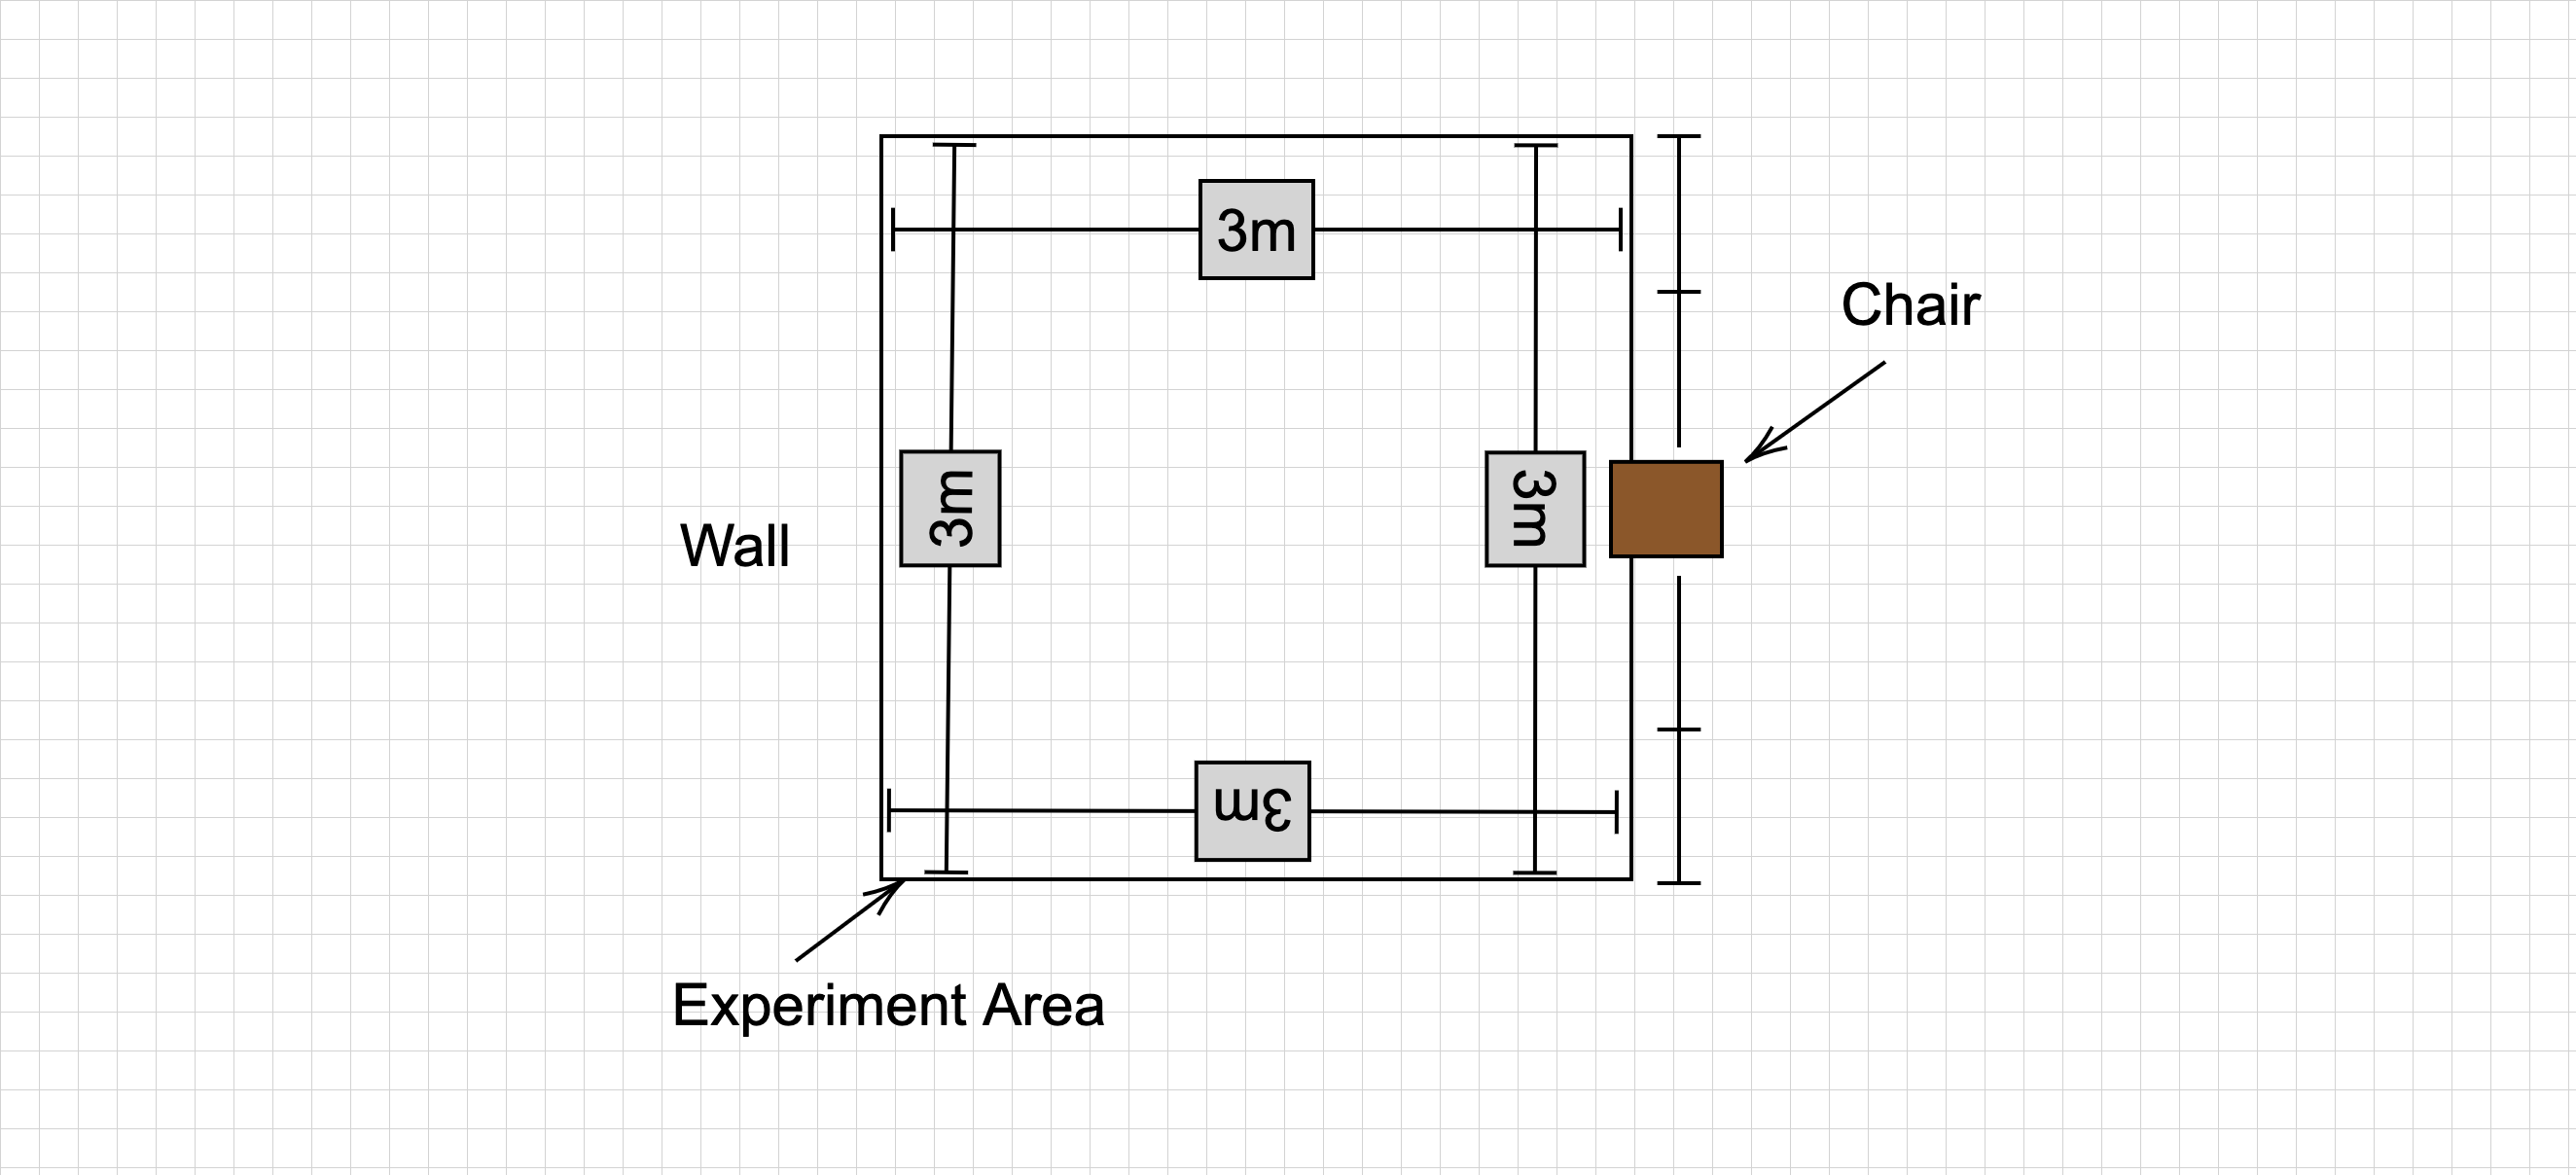
\includegraphics[scale=0.10]{graphics/experiment-diagram.png}
    \caption{The area designated to run the experiment}
    \label{Experiment}
\end{figure}



\section{Data}
After following the procedures outlined in Section \ref{Procedure}, the following datasets were found:

\begin{table}[H]
    \centering
    \begin{tabular}{lllllllll}
    \rowcolor[HTML]{C0C0C0} 
    \cellcolor[HTML]{FFCC67}{\color[HTML]{333333} Ratio} & Trial 1 & Trial 2 & Trial 3 & Trial 4 & Trial 5 & Trial 6 & Average & Range \\
    \cellcolor[HTML]{FFCC67}{\color[HTML]{333333} 4:4} & 1.23 & 0.83 & 1.23 & 0.9  & 1.03 & 1.3  & 1.086666667  & 0.47 \\
    \cellcolor[HTML]{FFCC67}{\color[HTML]{333333} 3:5} & 0.56 & 1.13 & 0.4  & 0.63 & 0.63 & 0.9  & 0.8975       & 0.73 \\
    \cellcolor[HTML]{FFCC67}{\color[HTML]{333333} 2:6} & 0.7  & 0.53 & 0.56 & 1.23 & 0.93 & 0.33 & 0.7108333333 & 0.9  \\
    \cellcolor[HTML]{FFCC67}{\color[HTML]{333333} 1:7} & 0.97 & 0.9  & 0.8  & 0.7  & 1.03 & 0.86 & 0.795        & 0.33 \\
    \cellcolor[HTML]{FFCC67}{\color[HTML]{333333} 0:8} & 0.77 & 0.93 & 0.96 & 0.86 & 0.86 & 0.96 & 0.89         & 0.19
    \end{tabular}
    \caption{The collected data.}
    \label{Data}
    \end{table}

\begin{figure}[H]
    \centering
    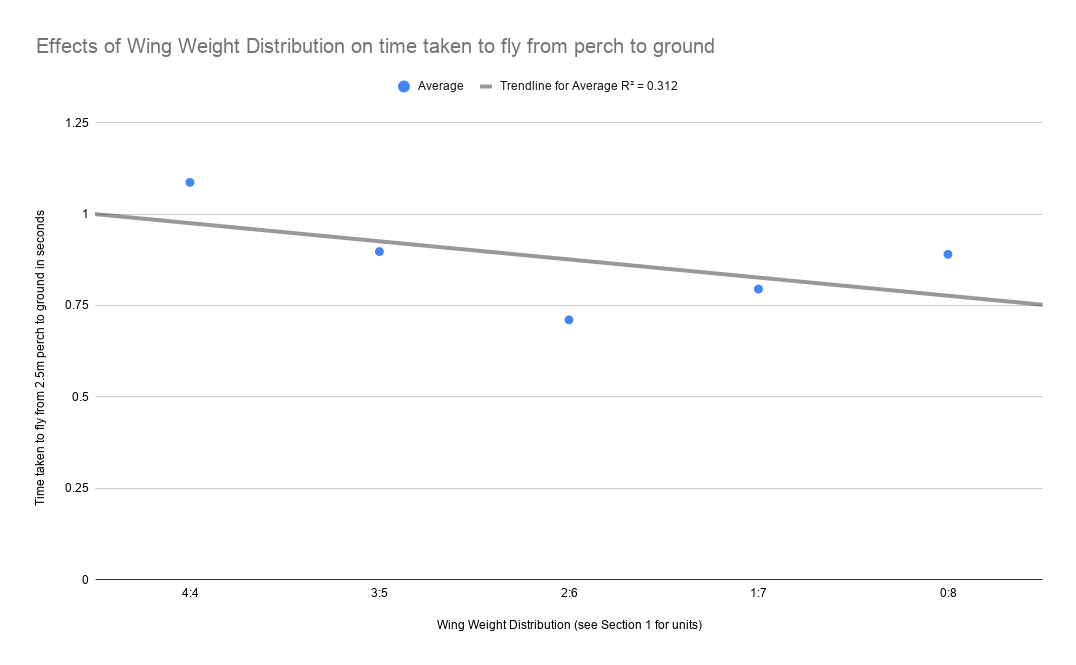
\includegraphics[scale=0.35]{graphics/graph-linear.png}
    \caption{Graph comparing average time taken to fly from starting point to ground and wing weight ratio with a linear model}
    \label{Linear Chart}
\end{figure}

\begin{figure}[H]
    \centering
    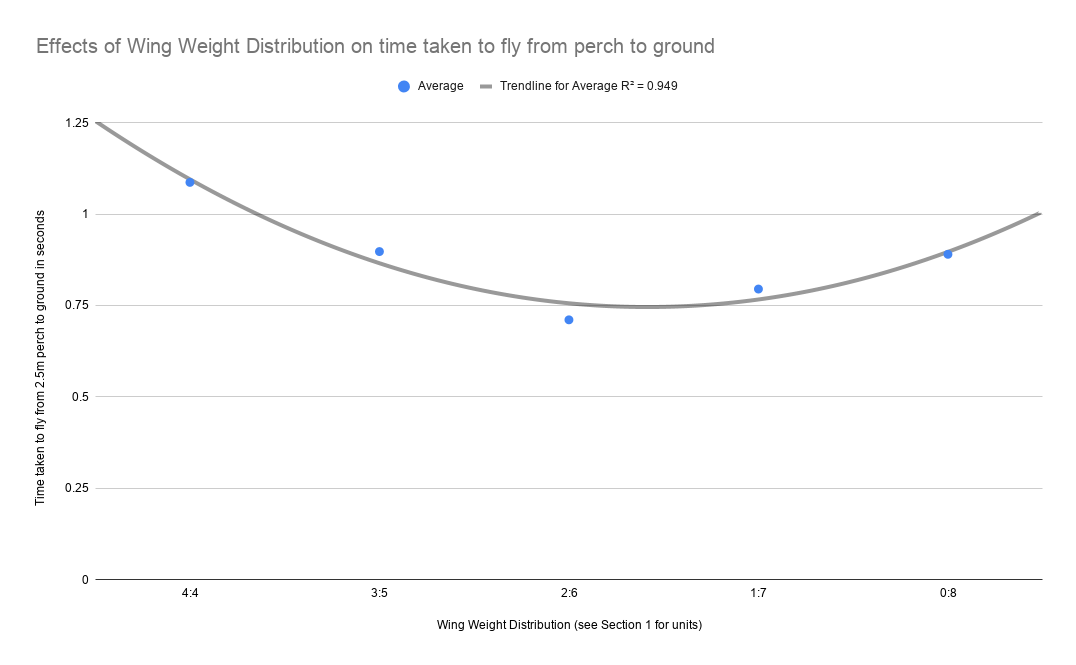
\includegraphics[scale=0.35]{graphics/graph-quadratic.png}
    \caption{Graph comparing average time taken to fly from starting point to ground and wing weight ratio with a polynomial model}
    \label{Quadratic Chart}
\end{figure}

\href{https://drive.google.com/open?id=1pxjHiAVFEnyUj759QoK4n0mFYVah-jPS}{Recorded Footage for Qualitative Analysis} \label{Qualitative Data Footage}

\subsection{Uncertainties}
Each of the data points have an absolute uncertainty of $\pm 0.01$s. This is a direct result of the frame-by-frame analysis described in the procedure, which required footage shot at a given framerate. However, video recordings each have miniscule delays in capturing each frame, and this was factored into the data, to create an uncertainty of $\pm 0.01$s.

There was also an absolute uncertainty of $0.005$m in the measuring of the height of the area used for the experiment. The experimenters used a relatively imprecise metre stick with increments in centimetres for the measuring of the total height of the space, which led to this calculation. 

\section{Discussion}

\subsection{Results and Analysis}

\subsubsection{Fitting the model and initial comparison with hypothesis}
It was initially hypothesized that as the wing weight ratio of a rotocopter was decreased, the flight time would also decrease. In other words, plotting the average flight time of a given rotocopter against its wing weight ratio should reveal a negative, linear correlation. This hypothesis was partially supported in the graphs; in Figure 4, it can be seen that the line of best fit (hereon referred to as the LOBF) followed this pattern of a decreasing negative correlation. The data in both Table \ref{Data} and Figure \ref{Linear Chart} showcase this fact, as each of the times are decreasing in correlation with a lower wing-weight ratio. However, the $R^2$ value of the LOBF in Figure \ref{Linear Chart} was about $0.3$, which means that it had an accuracy measurement of $\pm 30\%$. This was an unacceptable value to draw conclusions from, thus necessitating an adjustment to the LOBF. The experimenters changed the modelling equation from a linear model to a polynomial one of degree $2$, as there was a dip in the data at the $2:6$ ratio measurement. After this was done, the $R^2$ value jumped up to $0.95$, meaning that it was a much more accurate model, as can be seen by the closeness of the points to the curve in Figure \ref{Quadratic Chart}.

\subsubsection{Qualities of Polynomial Curve}
Because of the jump in the $R^2$ value with the second curve, the polynomial curve was deemed to be the best representation of the data at hand. Analyzing this curve, one can see that there is an 'optimal value' of the graph, whose y-value represents the time taken for the rotocopter to reach the ground, and the x-value representing the ratio of the weight of the left wing to the weight of the right. Coming back to the main point, this graph and optimized data only partially proves the hypothesis. It was stated that there would be a negative \textit{linear} correlation. The graph proves that there is a point at which the speed simply cannot be increased anymore; in other words, there is a minimum value. This point is further discussed in \ref{Qualitative Data}. This quadratic relation also showed that the two maximum values of the data set were the two extreme ratios; the wing weight ratios of 0:8 and 4:4, with their evaluated values being 0 and 1, respectively.

\subsubsection{Qualitative Data and Observations} \label{Qualitative Data}
Note: All files discussed in this section can be found in \href{https://drive.google.com/open?id=1pxjHiAVFEnyUj759QoK4n0mFYVah-jPS}{Recorded Footage for Qualitative Analysis}

The findings in the quantitative data were supported by the visuals found in the qualitative data. At the beginning of the procedure, when the testing of control group began, it can be seen that the rotocopter is spinning and gliding down at a relatively low speed (See file \verb|IMG_3695.mov|), and this effect is mimicked in the later stages of the experiment. In the testing of the last ratio (8 staples on the left wing, 0 on the right), it can be seen that the rotocopter did not spin, but glided down at a rate similar to the first one. In the parabola shown in (graph), it can also be seen that the lowest time taken to fly from the starting point $2.5\pm0.005$m in the air to the landing point on the ground was achieved by the rotocopter with wing ratios of $2:6$, which was perfectly in the middle of all the trials, which took about $0.71$seconds. In the footage (See file \verb|IMG_3715.mov|), it can be seen that the rotocopter with wing ratios of $2:6$ simply fell to the ground, as opposed to gracefully gliding down to the surface in the same manner as the other trials.

\subsection{Possible Errors}
Despite the data being quite precise (the ranges in Figure 4 are all relatively small), there could still have been both systematic and random errors made in the collection process, which might have skewed the data.

\label{Systematic Errors}
\subsubsection{Systematic}

The data collection method of choice was technological by nature, and this technology, however developer, still may have caused some systematic errors in measurement. For the initial experiment, the experimenters used a 2019 iPhone XR camera, which shot at approximately 30 frames per second, at a resolution of 1080p. This means that every $\frac{1}{30}$ seconds, a moment in time is captured. In some cases, the time that the rotocopter first touched the ground was in between these $\frac{1}{30}$ second increments, which could've skewed the final data. In addition to this, there is a certain amount of delay between the pressing of the 'start recording' button and the time that the camera actually starts recording. This delay in time, coupled with the framing issue, means that the margin of error is increased.

\subsubsection{Random}
As a result of averaging the values, many of the random errors were filtered out. However, there were still some random errors in the experiment.

One possible error could've been in the process of creating the rotocopters themselves. Each of the rotocopter templates required precise measurements and cutting of the paper, and owing to the rotocopter's small size, any miniscule mistake would have relatively large implications. For instance, if there was a rip in the paper around the centre of the copter, then air would be able to flow through that space, allowing the object to drop down faster.

Continuing on the point of human error, mistakes could also have been made in the experimentation process. The procedure states that humans dropped and interacted with all of the experimental objects. Humans can clearly see objects down to ~0.026mm when the object is ~15cm away from the eye in question (cite). As such, the process of dropping the rotocopter from a fixed height was not entirely precise. This problem of human accuracy could also have translated in the data collection of the experiment, through the time that the recording of footage began. In the procedure, it is noted in step 23 that the recording of the trial was started as soon as the person standing on the chair dropped the rotocopter \textit{and} said, "Go" or some other keyword. As a result, this part of the experiment relied mostly on the reflex time of each of the individuals conducting the experiment; the person dropping the copter had to react to their own dropping of the rotocopter, then say a keyword, then have the individual who is recording react to the keyword, and then start recording. Each of these steps take place in succession, adding to the amount of time it takes for the rotocopter to reach the ground, and skewing the results.

Another major factor affecting flight is wind, as it pushes air at either a greater or lower speed, depending on the type. This affects flight time readings for small objects much more; as a result of their small mass, objects like paper rotocopters are much more finicky. Although the experiment was conducted in a section of a hallway, there were still numerous possible sources of wind. In the experiment space, there were doors that were being opened and closed repeatedly, whose motion could've caused wind. In addition, the experimenters did not have any coverings over their mouths, so heavy breathing could've also affected the measurements through the air produced.

\subsection{Improvements}
As was demonstrated by the high amount of possible systematic and random errors in the experiment, there were numerous ways that the experiment could've been improved, starting with the human interactions. Obviously, our bodies are not necessarily suited to measure items with precision, so if this experiment were to be repeated, the humans would need to be replaced by machines, and more accurate devices. For instance, a robot arm could be used instead of a human to drop the rotocopter, ensuring a constant drop height. This arm could also be linked to the record button on the camera, or be linked to an automation system that starts recording on drop.

The framerate issue discussed in Section \ref{Systematic Errors} could've been solved by using a better camera, with a higher framerate, so as to capture more images at more times, increasing precision and decreasing the likelihood that the correct time was not captured.

The room could also have been a more closed space, with the measurements of 3m $\times$ 3m $\times$ 2.5m being the measurements of the room, and the experiment taking place inside of the room, so as to not have any outside disturbances, like wind, as stated previously.

\section{Conclusion}
In conclusion, the purpose of this experiment was to understand the effects of weight distribution of the wings of a rotocopter, between wing weight ratios ranging from $4:4$ to $0:8$, on the time taken to fly from one point 2.5m above the ground to the ground. This was done by stapling a total of 8 staples to the wings of the rotocopters, 2$\pm$0.05cm away from a given wing's edge, with each trial having a different wing weight ratio, and each wing's weight being 1 less or more than the one before it. When the times were noted down and compared with the ratios, they only partially supported the initial hypothesis, which stated that the flight times would go down as the wing weight ratio was decreased, creating a negative \textit{linear} correlation when the averages were plotted on a graph. This is because the graph displayed a quadratic model, rather than a linear one. This graph had an optimal value when the wing weight ratio of the rotocopter was at 2:6, whose flight time was about 0.71s. The experimenters ran the experiment primarily using human interaction, which led to a variety of random and systematic errors, but all of which could be fixed with better, more refined equipment.

\newpage

\section{Works Cited}

\begin{itemize}
    \item Ailerons. (n.d.). Retrieved from https://www.grc.nasa.gov/www/k-12/airplane/alr.html
    \item Anonymous. (n.d.). Factors Affecting Lift. Retrieved from https://howthingsfly.si.edu/aerodynamics/factors-affecting-lift
    \item Cutler, C. (2019, February 12). Why Does Stall Speed Increase With Bank Angle? Retrieved from https://www.boldmethod.com/learn-to-fly/aerodynamics/why-does-aircraft-stall-speed-increase-with-bank-angle/
    \item Dunbar, B. (2015, May 27). What Is a Helicopter? Retrieved from https://www.nasa.gov/audience/forstudents/5-8/features/nasa-knows/what-is-a-helicopter-58.html
    \item Random vs Systematic Error. (n.d.). Retrieved from https://www.physics.umd.edu/courses/Phys276/Hill/Information/Notes/ErrorAnalysis.html
\end{itemize}

\end{document}